\documentclass[a4paper,12pt]{article}
\usepackage[utf8]{inputenc}
\usepackage[ngerman]{babel}
\usepackage[a4paper, left=2.5cm, right=2.5cm]{geometry}
\usepackage{graphicx}
\usepackage{subcaption}
\usepackage{fancyhdr}
\usepackage{pdfpages}
\pagestyle{fancy}
\usepackage{multirow}
\usepackage{amsmath}
\lhead{Messtechnik Labor}
\chead{}
\rhead{Gruppe 2}

\begin{document}
	%Titelseite
	
\includepdf{tp4.pdf}
	
	\noindent
	\textbf{\Large Rechtliches} \\ \\
	Ich bestätige hiermit, dass alle hier verwendeten Messergebnisse und Interpretationen von uns selbst erstellt wurden. Es wurden keine anderen Quellen als die hier schriftlich angegeben verwendet.
	
	\newpage
	\tableofcontents
	
	\newpage
	\section{Einleitung}
	In dieser Laborübung verschiedene Übertragungsarten untersucht und getestet werden. Außerdem Störungen, Reflexionen und der SNR (Signal-Noise-Ratio) und deren Einfluss auf die Messung untersucht werden.
	
	\section{Übungsdurchführung}
	\subsection{Signalübertragung bei ungestörten Drahtleitungen}
	In diesem Teil der Laborübung soll die Übertragung von Signal auf Drahtleitungen untersucht werden.
	\subsubsection{Messaufbau}
	\begin{figure}[h]
		\centering
		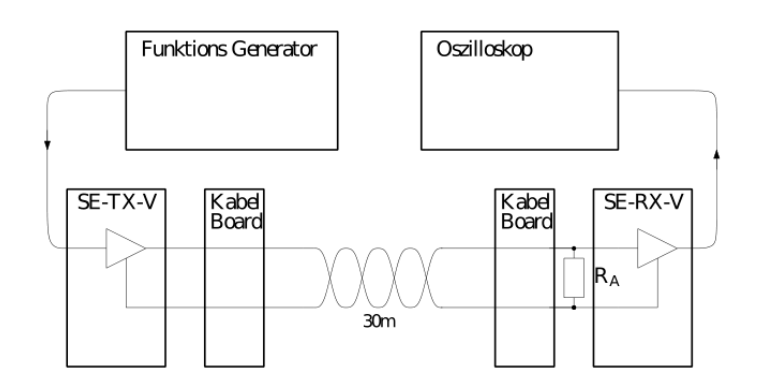
\includegraphics[width=15cm]{img/Messaufbau_2_1}
		\caption{Laboraufbau für 2.1}
	\end{figure}
	\noindent
	Dieser Messaufbau wird für die nächsten beiden Messungen benötigt. Der einzige Unterschied zwischen den beiden Messungen werden die Einstellungen am Funktionsgenerator sein.
	\newpage
	\subsubsection{Reflexionen}
	\underline{\textbf{Aufgabenstellung}} \\ \\
	Hier soll der Einfluss von verschiedenen Abschlusswiderständen auf die Signalübertragung untersucht werden. \\ \\
	\underline{\textbf{Durchführung}} \\ \\
	Zunächst wurden zuerst am Funktionsgenerator folgende Einstellungen getätigt:
	\begin{table}[h]
		\centering
		\begin{tabular}{|c|c|c|c|}
			\hline
			\multirow{2}{*}{\textbf{Amplitude}} & \multirow{2}{*}{\textbf{Offset}} & \multirow{2}{*}{\textbf{Frequenz}} & \multirow{2}{*}{\textbf{Signalform}} \\
			&  &  &  \\ \hline
			\multirow{2}{*}{$100mV_{pp}$} & \multirow{2}{*}{$4V$} & \multirow{2}{*}{$10kHz$} & \multirow{2}{*}{Rechteck} \\
			&  &  &  \\ \hline
		\end{tabular}
		\caption{Einstellungen des Funktionsgenerators für die Reflexionsmessung}
	\end{table}
	\newline
	Das eingespeiste Signal soll über ein 30m langes Kabel übertragen werden. Dieses übertragene Signal soll wiederum mit einem Oszilloskop aufgenommen werden. Die Abschlusswiderstände sollen bei dieser Messung variiert werden um auftretende Unterschiede zu untersuchen.
	\begin{figure}[h]
		\centering
		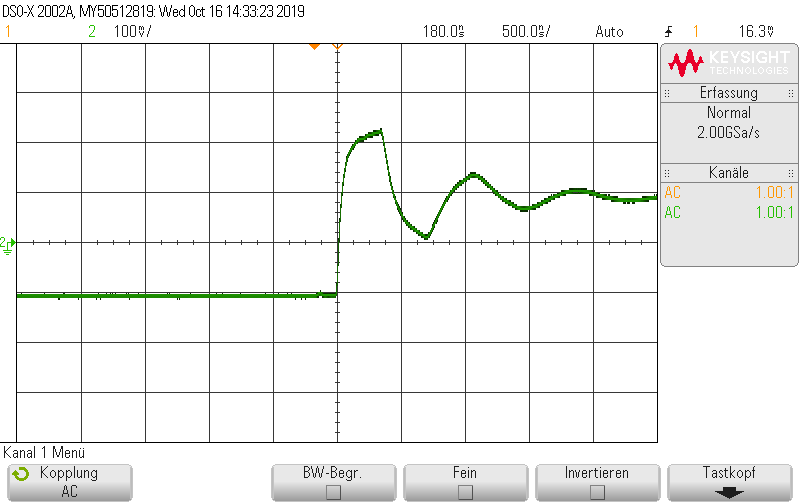
\includegraphics[width=12cm]{img/RA_unendlich}
		\caption{Ausgang bei R\textsubscript{$A$} gleich $\infty$}
	\end{figure}
	\newpage
	\begin{table}[h]
		\centering
		\begin{tabular}{|c|c|c|c|}
			\hline
			\multicolumn{1}{|c|}{\multirow{2}{*}{$R_A[\Omega]$}} & \multirow{2}{*}{$|V_{1,peak}|[mV]$} & \multirow{2}{*}{$|V_{2,peak}|[mV]$} & \multirow{2}{*}{$\Delta t_{peaks}[ns]$} \\
			\multicolumn{1}{|c|}{} &  &  &  \\ \hline
			\multirow{2}{*}{$\infty$} & \multirow{2}{*}{$123.25$} & \multirow{2}{*}{$82.5$} & \multirow{2}{*}{$360$} \\
			&  &  &  \\ \hline
			\multirow{2}{*}{$50$} & \multirow{2}{*}{$36.87$} & \multirow{2}{*}{$5.625$} & \multirow{2}{*}{$360$} \\
			&  &  &  \\ \hline
			\multirow{2}{*}{$100$} & \multirow{2}{*}{$1.250$} & \multirow{2}{*}{$0$} & \multirow{2}{*}{$360$} \\
			&  &  &  \\ \hline
			\multirow{2}{*}{$200$} & \multirow{2}{*}{$38.5$} & \multirow{2}{*}{$10$} & \multirow{2}{*}{$360$} \\
			&  &  &  \\ \hline
		\end{tabular}
		\caption{Auswertung der Refelxionsmessung}
	\end{table}
	\noindent
	Aus Tabelle 2 ist klar ersichtlich, das der Leitungswellenwiderstand $Z_L$ $100\Omega$ betragen muss, weil wird die Leitung mit einen Abschlusswiderstand von $50\Omega$ abgeschlossen, treten die wenigsten Reflexionen am Ausgang auf. Dies ist in Abbildung 3 zu erkennen.
	\begin{figure}[h]
		\centering
		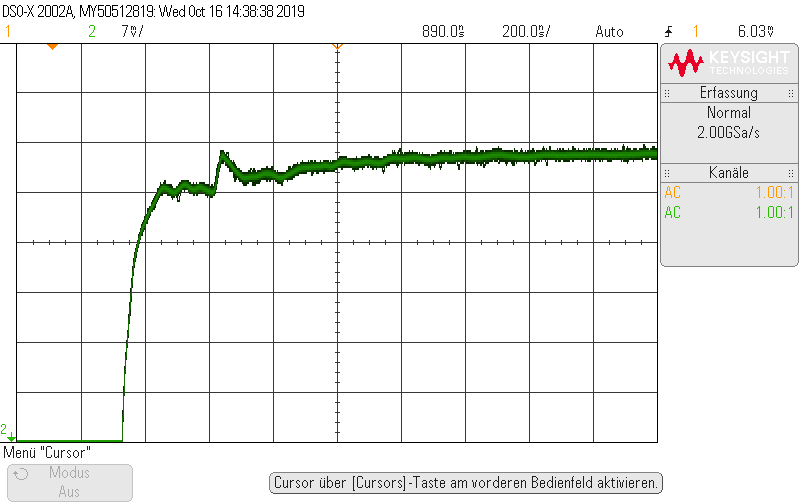
\includegraphics[width=13cm]{img/Ra100}
		\caption{Ausgang bei R\textsubscript{$A$} gleich $50\Omega$}
	\end{figure}
	\newpage
	\subsubsection{Berechnung der Dämpfung des Kabels}
	Es wird angenommen, dass die Ausgangsspannung des Kabels entsprechend 
	\newline
	$U(z) = U(0)e^{-\alpha z}$ abnimmt. Am besten zur Bestimmung der Dämpfung des Kabels eignen sich die Messergebnisse bei unendlichen Abschlusswiderstand. $|V_{1,peak}|$ entspricht dem Wert $U(0)$ und $|V_{2,peak}|$ entspricht $U(60)$. $U(60)$ deswegen, weil die Reflexion die doppelte Kabellänge zurücklegen muss. Nun kann $\alpha$ bestimmt werden.
	\begin{align*}
		U(60) &= U(0) \ast e^{-\alpha \cdot 60} \\
		\alpha &= -\frac{\ln\left( \frac{U(60)}{U(0)}\right)}{60} = 8.36 \cdot 10^{-3}
	\end{align*}
	Da nun $\alpha$ bestimmt ist, kann nun die gewünschte Dämpfung wie folgt berechnet werden.
	\[
		\frac{U(100)}{U(0)} = e^{-\alpha\cdot 100} = 0.4333 = -7.2627dB
	\]
	Außerdem kann auch die Ausbreitungsgeschwindigkeit des Signals über das Kabel berechnet werden:
	\[
		c = \frac{l}{\Delta t_{peaks}} = \frac{60m}{360ns} = 1.667 \cdot 10^8
	\]
	Dies entspricht dem $0.55$-fachen der Lichtgeschwindigkeit $c_0$.
	\subsubsection{Bandbreite}
	\underline{\textbf{Aufgabenstellung}} \\ \\
	Es soll die 3dB-Bandbreite des Übertragungssystem aus Abbildung 1 bestimmt werden. \\ \\
	\underline{\textbf{Durchführung}} \\ \\ 
	In Tabelle 3 sieht man die Einstellungen, die man beim Frequenzgenerator tätigen muss, um diese Messung durchführen zu können.
	\begin{table}[h]
		\centering
		\begin{tabular}{|c|c|c|c|}
			\hline
			\multirow{2}{*}{\textbf{Amplitude}} & \multirow{2}{*}{\textbf{Offset}} & \multirow{2}{*}{\textbf{Frequenz}} & \multirow{2}{*}{\textbf{Signalform}} \\
			&  &  &  \\ \hline
			\multirow{2}{*}{$100mV_{pp}$} & \multirow{2}{*}{$4V$} & \multirow{2}{*}{$100kHz - 10MHz$} & \multirow{2}{*}{Sinus} \\
			&  &  &  \\ \hline
		\end{tabular}
		\caption{Einstellungen des Funktionsgenerators für 2.1.4}
	\end{table}
	\newpage
	\noindent	
	Es wird die Frequenz des Eingangsignales so lange erhöht, bis die Beziehung 
	\newline
	$U_a = \frac{1}{\sqrt{2}} \ast U_e$ gültig ist, denn dies entspricht einer Verstärkung von -3dB. Die eingestellte Frequenz, die diese Bedingung erfüllt ist dann die Grenzfrequenz bzw. die Bandbreite des Übertragungssystem. Diese wurde als 4.56 MHz bestimmt.
	\subsection{Signalübertragung über einen gestörten Kanal}
	In diesem Teil wird über den gerade aufgebauten Kanal auch ein Störsignal übertragen und dessen Einwirkungen auf das Nutzsignal untersucht.
	\subsubsection{Bestimmung des Signal-to-Noise Ratios}
	\begin{figure}[h]
		\centering
		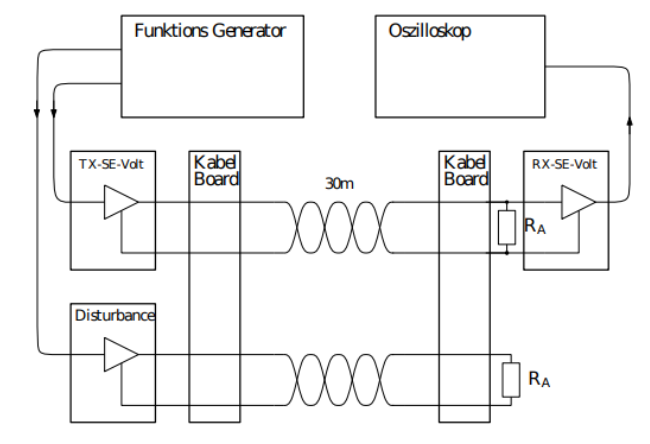
\includegraphics[width=12cm]{img/Laboraufbau2_2_1}
		\caption{Laboraufbau für Aufgabe 2.2.1}
	\end{figure}
	\noindent
	Sowohl das Nutzsignal auch als das Störsignal wird vom Funktionsgenerator erzeugt. Die zu wählenden Einstellungen sind in folgender Tabelle zu sehen.
	\newpage
	\begin{table}[h]
		\centering
		\begin{tabular}{|c|c|c|c|c|}
			\hline
			\multirow{2}{*}{} & \multirow{2}{*}{\textbf{Amplitude}} & \multirow{2}{*}{\textbf{Offset}} & \multirow{2}{*}{\textbf{Frequenz}} & \multirow{2}{*}{\textbf{Signalform}} \\
			&  &  &  &  \\ \hline
			\multirow{2}{*}{Sender} & \multirow{2}{*}{$-$} & \multirow{2}{*}{$4V$} & \multirow{2}{*}{$-$} & \multirow{2}{*}{DC} \\
			&  &  &  &  \\ \hline
			\multirow{2}{*}{Störsender} & \multirow{2}{*}{$3V_{pp}$} & \multirow{2}{*}{$2V$} & \multirow{2}{*}{$10MHz$} & \multirow{2}{*}{Noise} \\
			&  &  &  &  \\ \hline
		\end{tabular}
	\caption{Einstellungen des Funktionsgenerator für 2.2.1}
	\end{table}
	\noindent
	Der RMS des Rauschsignal $U_{R,eff}$ wurde als $11.73mV$ bestimmt. Desweiteren betrug der Effektivwert des gesamten Ausgangsignals betrug $4V$. Das SNR lässt sich nun wie folgt bestimmen:
	\[
		SNR_{dB} = 20 \cdot \log \left( \frac{U_{a,eff}}{U_{R,eff}}\right) = 50.65dB
	\]
	Um einen SNR von $0dB$ zu erreichen, müssen die Effektivwerte des Nutz- und Rauschsignales gleich sein.
	Würde man ein Sinussignal mit $10kHz$ am Eingang legen müsste dieses eine Amplitude von $16.598mV$ besitzen um einen SNR von $0dB$ am Ausgang zu erreichen.
	\[
		\hat{U}_N = \sqrt{2} \cdot U_{N,eff} = \sqrt{2} \cdot U_{R,eff}
	\]
	Anschließend wurde die FFT (Fast Fourier Transformation)-Funktion des Oszilloskop verwendet, um das Spektrum des Rauschsignales zu untersuchen.
	\begin{figure}[h]
		\centering
		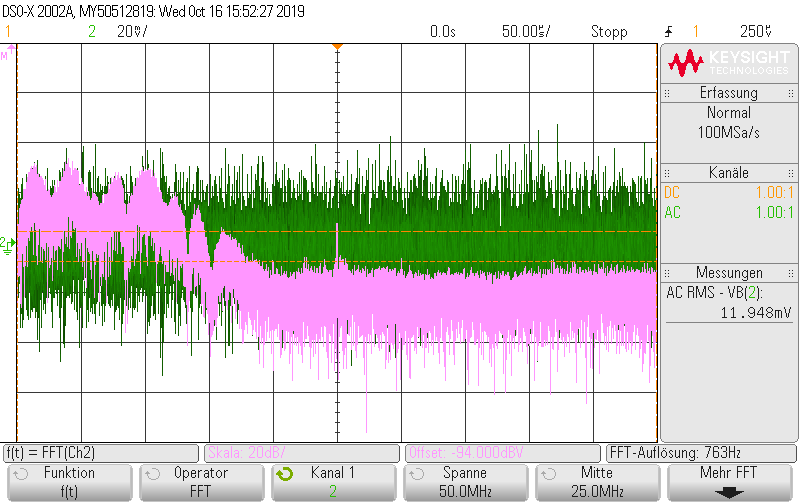
\includegraphics[width=13cm]{img/FFT}
		\caption{Spektrum des Rauschens}
	\end{figure}
	\newline
	Will man nun das SNR steigern, jedoch ohne das Nutzsignal zu erhöhen, kann entweder ein Tiefpass vor den Eingang geschaltet werden, um das Rauschen, welches großteils höher frequent ist als das Nutzsignal ist, herauszufiltern. Ein weitere Möglichkeit besteht darin die Übertragung differentiell durchzuführen. \\ \\
	\textbf{Tiefpass:} \\ \\
	\begin{figure}[h]
		\centering
		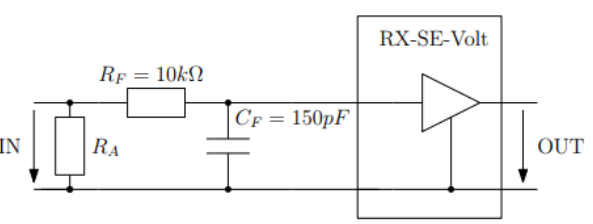
\includegraphics[width=15cm]{img/Tiefpass}
		\caption{Integrierter Tiefpass}
	\end{figure}
	\newline
	Die Grenzfrequenz dieses Tiefpasses lässt sich wie folgt bestimmen:
	\[
		f_C = \frac{1}{2\pi R_F C_F} = 106.103kHz
	\]
	Mit diesen vorgeschalteten Tiefpass konnte der RMS des Rauschen auf $609\mu V$ reduziert werden. Dies führt zu einen SNR von $76.34dB$. Anschließend wurde wieder die 3dB-Bandbreite bestimmt. Diese betrug nun 85kHz. \\
	Anhand dieser Messergebnisse kann man daraus schließen, dass das zu entwerfende Messsystem nicht einen hohen SNR und eine große Brandbreite besitzen kann. Daher muss beim Entwurf eines Messsystems also immer Überlegungen getroffen werden, welche Art von Signalen man übertragen möchte, bevor man einen Filterung durchführt. Dadurch könnte man nämlich das Messsignal verfälschen.
	\newpage
	\subsubsection{Differentiele Übertragung}
	In diesem Teil des Labors sollen die Unterschiede zwischen der single-ended und der differentiellen Übertragung untersucht werden. Der Unterschied von differentieller zur single-ended Übertragung besteht darin, dass das Nutzsignal ebenfalls invertiert und auf einer zweiten Leitung übertragen wird. Störungen werden auf beide Signale überlagert und können dann anschließend mit einen Differenzverstärker wieder entfernt werden.
	\begin{figure}[h]
		\centering
		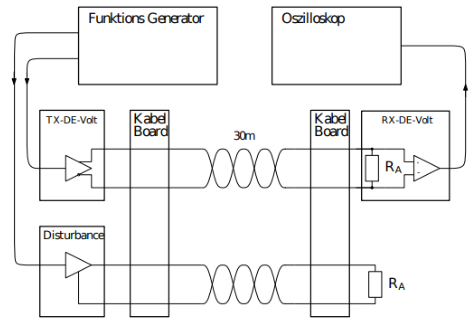
\includegraphics[width=12cm]{img/Laboraufbau2_2_2}
		\caption{Laboraufbau von 2.2.2}
	\end{figure}
	\newline
	Die folgenden Einstellungen wurden am Funktionsgenerator getätigt:
	\begin{table}[h]
		\centering
		\begin{tabular}{|c|c|c|c|c|}
			\hline
			\multirow{2}{*}{} & \multirow{2}{*}{\textbf{Amplitude}} & \multirow{2}{*}{\textbf{Offset}} & \multirow{2}{*}{\textbf{Frequenz}} & \multirow{2}{*}{\textbf{Signalform}} \\
			&  &  &  &  \\ \hline
			\multirow{2}{*}{Sender} & \multirow{2}{*}{$-$} & \multirow{2}{*}{$0.5V$} & \multirow{2}{*}{$-$} & \multirow{2}{*}{DC} \\
			&  &  &  &  \\ \hline
			\multirow{2}{*}{Störsender} & \multirow{2}{*}{$3V_{pp}$} & \multirow{2}{*}{$2V$} & \multirow{2}{*}{$10MHz$} & \multirow{2}{*}{Noise} \\
			&  &  &  &  \\ \hline
		\end{tabular}
		\caption{Einstellungen des Funktionsgenerator für 2.2.2}
	\end{table}
    \newline
	Wird die Signalübertragung differentiell durchgeführt wurde ein RMS des Rauschen von $962\mu V$ gemessen. Um  ein SNR von $0dB$ am Ausgang zu erreichen, wenn man ein Sinussignal von 10kHz am Eingang anlegt, muss dieses eine Amplitude von $1.36mV$ besitzen. Da die Störung sowohl bei der single-ended als auch bei der differentiellen Übertragung die gleiche ist, kann man leicht einen Vergleich durchführen.
	\newpage
	\noindent
	Die differentielle Übertragung senkt den RMS des Rauschens um den Faktor $12.19$ besser als wie die single-ended Übertragung. Dadurch ist ersichtlich das die differentielle Signalübertragung eine gute Methode ist, um das SNR eines Messsystems zu erhöhen.
	
	\subsubsection{Analog-Digital Wandlung}
	Eine weitere Alternative um das Nutzsignal resistenter gegen Störungen zu machen, ist es vor der Übertragung des Signales in ein digitales Signal umzuwandeln. Die benötigte Bitrate wird folgendermaßen berechnet:
	\[
		Bitrate = Samplerate \cdot Bitzahl = 100kSPS \cdot 16bit = 1.6Mbps
	\]
	\begin{table}[h]
		\centering
		\begin{tabular}{|c|c|c|c|c|}
			\hline
			\multirow{2}{*}{} & \multirow{2}{*}{\textbf{Amplitude}} & \multirow{2}{*}{\textbf{Offset}} & \multirow{2}{*}{\textbf{Frequenz}} & \multirow{2}{*}{\textbf{Signalform}} \\
			&  &  &  &  \\ \hline
			\multirow{2}{*}{Sender} & \multirow{2}{*}{$3V_{pp}$} & \multirow{2}{*}{$1.5V$} & \multirow{2}{*}{$1.6Mbps$} & \multirow{2}{*}{PRBS} \\
			&  &  &  &  \\ \hline
			\multirow{2}{*}{Empfänger} & \multirow{2}{*}{$3V_{pp}$} & \multirow{2}{*}{$2V$} & \multirow{2}{*}{$10MHz$} & \multirow{2}{*}{Noise} \\
			&  &  &  &  \\ \hline
		\end{tabular}
		\caption{Einstellungen des Funktionsgenerator für 2.2.3}
	\end{table}
	\newline
	Nun soll das Augendiagramm des Empfängers am Oszilloskop dargestellt werden. Dies wird mit einem Trigger, der auf beide Flanken regiert, und auf ein Nachleuchten im Oszilloskop realisiert.
	\begin{figure}[h]
		\centering
		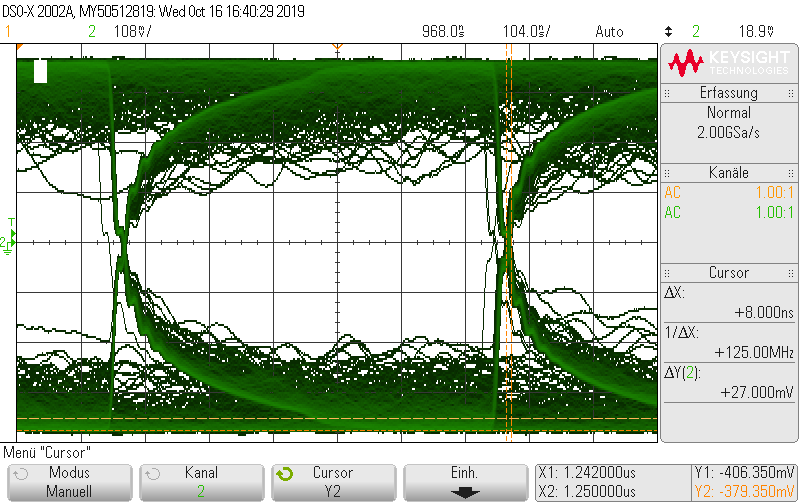
\includegraphics[width=10.5cm]{img/Augendiagramm}
		\caption{Augendiagramm}
	\end{figure}
	\newpage
	\begin{table}[h]
		\centering
		\begin{tabular}{|c|c|c|}
			\hline
			\multirow{2}{*}{1} & \multirow{2}{*}{Bitrate[Mbps]} & \multirow{2}{*}{$1.6$} \\
			&  &  \\ \hline
			\multirow{2}{*}{2} & \multirow{2}{*}{$U_1$ Spannungslevel bei digial 1 [mV]} & \multirow{2}{*}{$391.5$} \\
			&  &  \\ \hline
			\multirow{2}{*}{3} & \multirow{2}{*}{$U_0$ Spannungslevel bei digital 0 [mV]} & \multirow{2}{*}{$-406.35$} \\
			&  &  \\ \hline
			\multirow{2}{*}{4} & \multirow{2}{*}{Anstiegszeit[ns]} & \multirow{2}{*}{$52$} \\
			&  &  \\ \hline
			\multirow{2}{*}{5} & \multirow{2}{*}{Abfallszeit[ns]} & \multirow{2}{*}{$78$} \\
			&  &  \\ \hline
			\multirow{2}{*}{6} & \multirow{2}{*}{Jitter des Übergangszeitpunktes 0-1 und 1-0 [ns]} & \multirow{2}{*}{$8$} \\
			&  &  \\ \hline
			\multirow{2}{*}{7} & \multirow{2}{*}{$\sigma_1$ Rauschen des Spannungslevel von 1[mV]} & \multirow{2}{*}{$21.6$} \\
			&  &  \\ \hline
			\multirow{2}{*}{8} & \multirow{2}{*}{$\sigma_2$ Rauschen des Spannungslevel von 0[mV]} & \multirow{2}{*}{$27$} \\
			&  &  \\ \hline
		\end{tabular}
		\caption{Auswertung des Augendiagrammes}
	\end{table}
	\noindent
	Des weiteren soll der Effektivwert des Rauschen berechnet werden, der zu einer BER (Bit Error Rate) von $10^{-9}$ führen würde. Der BER entspricht einen SNR von $21.6dB$.
	\[
		SNR_{dB} = 20 \cdot \log\left(\frac{U_1 - U_0}{U_{R,RMS}}\right)
	\]
	Nun kann der RMS des Rauschens berechnet werden.
	\[
		U_{R,RMS} = \frac{U_1 - U_0}{10^{\frac{SNR_{dB}}{20}}} = 66.28mV
	\]
	\newpage
	\subsection{Signalübertragung über Stromsignale}
	In diesem Teil der Laborübung soll die Signalübertragung mittels Stromsignalen untersucht werden. Der wesentliche Vorteil von Strom- gegenüber Spannungssignal ist, das ein Regler verwendet wird, der den Ausgangsstrom so einstellt, sodass Serienwiderstände kompensiert werden.
	\begin{figure}[h]
		\centering
		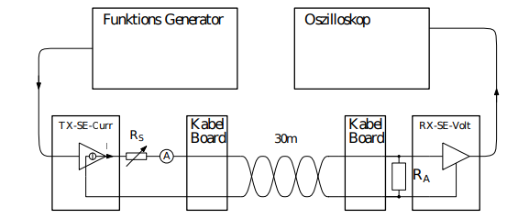
\includegraphics[width=15cm]{img/Laboraufbau2_2_3}
		\caption{Laboraufbau für 2.2.3}
	\end{figure}
	\newline
	Nun sollen sowohl die Sensitivität der bei Stromsignalen und Spannungssignalen ermittelt werden. Die Funktionsgeneratoreinstellungen lauten wie folgt:
	\begin{table}[h]
		\centering
		\begin{tabular}{|c|c|c|c|c|}
			\hline
			\multirow{2}{*}{} & \multirow{2}{*}{\textbf{Amplitude}} & \multirow{2}{*}{\textbf{Offset}} & \multirow{2}{*}{\textbf{Frequenz}} & \multirow{2}{*}{\textbf{Signalform}} \\
			&  &  &  &  \\ \hline
			\multirow{2}{*}{Sender} & \multirow{2}{*}{$5V_{pp}$} & \multirow{2}{*}{$2.5V$} & \multirow{2}{*}{$10kHz$} & \multirow{2}{*}{Sinus} \\
			&  &  &  &  \\ \hline
		\end{tabular}
		\caption{Einstellungen des Funktionsgenerator für 2.2.4}
	\end{table}
	\newline
	Der einstellbare Widerstand konnte bis zu $100\Omega$ betragen, wenn man in bis zum Anschlag gedreht hat. Auf Anweisung des Tutors wurden zur Ermittlung der Sensitivität immer nur 2 Werte bestimmt. Dies waren bei R\textsubscript{s} gleich $0\Omega$ und R\textsubscript{s} gleich $100\Omega$.
	\newpage
	\noindent
	\textbf{Stromsignal:}
	\begin{align*}
		R_s &= 0\Omega : 179mV \\
		R_s &= 100\Omega: 179mV \\
	\end{align*}
	Da man hier keine Änderung erkennen kann beträgt die Sensitivität $0 V/\Omega$. \\ \\
	\textbf{Spannungssignal:}
	\begin{align*}
		R_s &= 0\Omega : 2.075V \\
		R_s &= 100\Omega : 2.925V
	\end{align*}
	Die Sensitivität bei Spannungssignalen beträgt hier $0.0085 V/\Omega$.
	\section{Verwendete Geräte}
	\begin{itemize}
		\item Agilent 33500B (Funktionsgenerator)
		\item Agilent DSO-X-2002A (Digital Storage Oscilloscope)
		\item Agilent U1232A (True RMS Multimeter)
	\end{itemize}
	\newpage
	\listoffigures
	
	\newpage
	\listoftables
\end{document}